\documentclass[conference]{IEEEtran}
\usepackage{cite}
\usepackage{amsmath,amssymb,amsfonts}
\usepackage{algorithmic}
\usepackage{graphicx}
\usepackage{textcomp}
\usepackage{xcolor}
\def\BibTeX{{\rm B\kern-.05em{\sc i\kern-.025em b}\kern-.08em
    T\kern-.1667em\lower.7ex\hbox{E}\kern-.125emX}}

\begin{document}
\title{Survey on Aspect-Based Sentiment Analysis}

\author{\IEEEauthorblockN{Mohammad Ahmad}
\IEEEauthorblockA{\textit{Computer Science Dept. - HBG}\\
\textit{Pennsylvania State University}\\
Middletown, USA\\
mohammad.ahmad@psu.edu}
}

\maketitle
\thispagestyle{plain}
\pagestyle{plain}

\begin{abstract}
Aspect-based Sentiment Analysis (ABSA) is a very important field within Natural Language Processing (NLP). It has 2 major tasks which are Aspect Extraction (AE) and Aspect Sentiment Classification (ASC). With the increasing amount of reviews, blogs, articles, and other opinion-based texts which are produced for every possible entity such as places (restaurants, schools), food items, and products; there is no surprise that the stakeholders of these entities value the critical feedback and hope for efficient ways to analyze this large amount of feedback and opinions. From statistical models in the beginning to the neural models of today. From RNN based models to BERT based models. This field has experienced a wide array of techniques. These days we can see the attempt to move from Supervised and Semi-Supervised approaches to Unsupervised ones so that finally the promise of ABSA is realized; to extract aspect specific sentiments without being constrained by labeling and domain. In this paper, the many approaches that have been used over the years to perform ABSA will be explored so that we can derive an understanding and appreciation of how far we have come in our progress in this field.
\end{abstract}

\section{Introduction}
An important area of study within the field of Natural Language Processing (NLP) is Sentiment Analysis (SA). SA is defined as extracting the emotional tone or the expressed polarity in a given text. This is usually done by classifying a given text as expressing a positive, a negative, or a neutral sentiment. A further area of study within SA is Feature-Based or Aspect-Based Sentiment Analysis (ABSA). This refers to the extraction of expressed sentiments about the individual entities or objects within a text.

The motivation behind studying ABSA is simply that there is no scarcity in the amount of text containing opinions being produced. And it is often too simplistic of an approach to deem an entire text as expressing a positive, a negative, or a neutral opinion. The reality is that within an opinion piece, the writer is usually expressing opinions regarding multiple different aspects or subjects which then build up to the overall opinion being expressed by the text. Though it is valuable to find out the overall opinion being expressed by a text, it is more actionable for a concerned entity of an opinion piece to be able to extract the opinions about the individual aspects mentioned within the text.

Two important subtasks in ABSA are Aspect Extraction (AE) and Aspect Sentiment Classification (ASC). These subtasks have been the point of focus in many studies pertaining to ABSA since their introduction in SemEval 2014, a research workshop on NLP. AE is the subtask in ABSA which focuses on extracting the objects from a given text regarding which a sentiment is being expressed while ASC is the subtask which focuses on classifying the expressed sentiment for each aspect that was extracted.

The aim of this survey is to investigate the a small selection of papers from 4 time intervals and review those papers to ascertain the progress made in the field of ABSA.

\section{Paper Reviews}

\subsection{2020-2023}

\textit{\textbf{Adversarial Training for Aspect-Based Sentiment
Analysis with BERT, A. Karimi et al., 2020.}}

This paper talks about the idea of adversarial training, i.e. introducing noise or perturbations to input such that to a human it would seem as the same input with some noise but a neural network would perceive that as a completely different input and may not classify it correctly. This approach has already been used for sentence classification but not in ABSA.

\begin{figure}[htbp]
\centerline{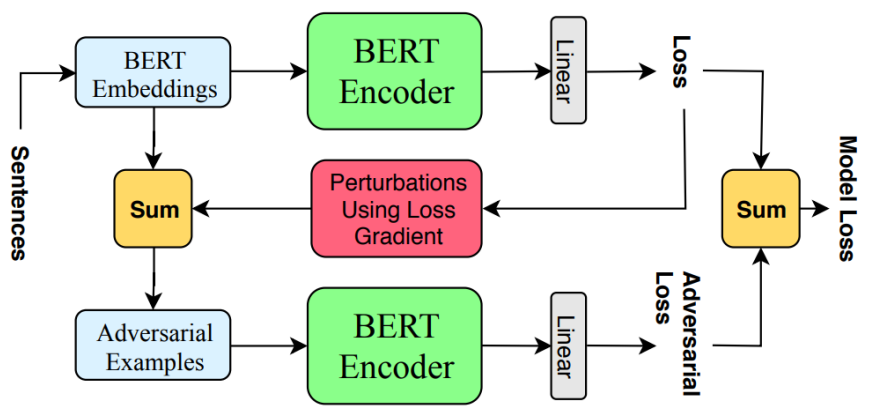
\includegraphics[keepaspectratio, width=0.45\textwidth]{pics/1.png}}
\caption{A representation of the model used by A. Karimi et al.}
\label{fig}
\end{figure}

\begin{figure*}
\centerline{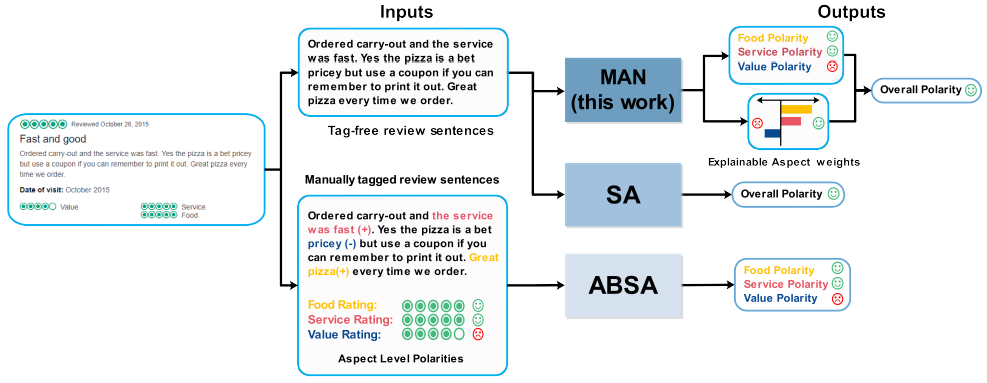
\includegraphics[keepaspectratio, width=\textwidth]{pics/2.png}}
  \caption{A summary of the aims of Y. Qiang at al in this paper.}
\end{figure*}

The models used in this paper is are extensions of the Bidirectional Encoder Representations from Transformers (BERT) model. The input sentences first go through a BERT word embedding layer to encode them. The encoded words are then passed through a BERT encoder following which their loss is calculated using a cross entropy loss function. After this the loss is used to calculate perturbations which are then added to the embeddings to produce input to attack the encoder and force it to give incorrect results. The adversarial loss and the normal loss are summed up to give the overall model loss, which is then minimized using backpropogation. A representation of this model is given by Figure 1. This model was used in both AE and ASC subtasks.

For the AE subtask, the goal was to assign each word a label so as to specify whether it is the beginning of an aspect, inside an aspect or not in any aspect. For the ASC subtask, the output from the previous subtask is used as input (in the evaluation stage, while the actual true values are utilized in training) with the modification that each text is repeated as many times as there are aspects in it so that the sentiment for each aspect can be classified separately.

The hyper-parameter to be optimized is the variable that controls how big the perturbations being added to the input sample are. The challenge with optimizing that was that the adversarial sample to be produced needed to be similar enough to the input to be classified as the same but also different enough from the input so as to challenge the model. The issue that the authors faced is that they were using 2 distinct datasets but the best value that they found was different for both meaning that the dataset itself influences the best value for this parameter.

Furthermore, as the authors were building upon another research on the same topic but using a post-trained BERT (BERT-PT), they had to keep many things in their paper and methodology consistent with that approach. This means that their paper is easy to compare with other approaches but it seems there was still room for further experimentation for their approach as it was constrained so as to be comparable.


\begin{table}[htbp]
\caption{Results of the model produced by Y. Qiang et al.}
\begin{center}
\begin{tabular}{|c|c|c|c|}
\hline
\multicolumn{2}{|c|}{\textbf{Restaurant}} & \multicolumn{2}{|c|}{\textbf{Laptop}} \\
\hline
\textbf{AE} & \textbf{ASC} & \textbf{AE} & \textbf{ASC} \\
\hline
80.9 & 85.4 & 85.6 & 78.1 \\
\hline
\end{tabular}
\end{center}
\end{table}

The model was trained and tested on the SemEval datasets from 2014 and 2016 which had restaurant and laptop reviews. It should be noted that many studies on AE and ASC use these datasets which makes these studies easier to compare with one another. As can be seen from Table 1, the results were indeed an improvement upon BERT-PT and it can be said that they had produced the best results at the time for the given datasets.\\

\textit{\textbf{Toward Tag-free Aspect Based Sentiment Analysis:
A Multiple Attention Network Approach, Y. Qiang et al., 2020.}}

This paper identifies the issue that datasets for ABSA need to have the aspects tagged manually, which leads to their being less relevant data available even though there is a very large number of review and opinion texts available online today. This is referred to as the cold-start problem. They propose a new Multiple-Attention Network (MAN) approach which crawls the review data from review websites to extract the tag-free review text, aspect-level ratings, and overall ratings. Their aim is to provide an end-to-end automatic solution to perform ABSA as well as to uncover the weighted contribution of each word towards the aspect-level and overall polarities. A summary of their aim is provided by Figure 2.

The contributions of this work are combating the cold-start for ABSA models by creating a means to produce datasets from review websites, providing 2 new datasets made from TripAdvisor, and including a means of inferring the overall sentiment from the aspect polarities by identifying the contribution of each aspect towards the overall score. The paper comments that a lot of ABSA approaches are built on SemEval Task 5, and the authors want a greater use of the massive online review data being generated from e-commerce websites by alleviating the laborious process of manually tagging the available reviews.

\begin{figure}[htbp]
\centerline{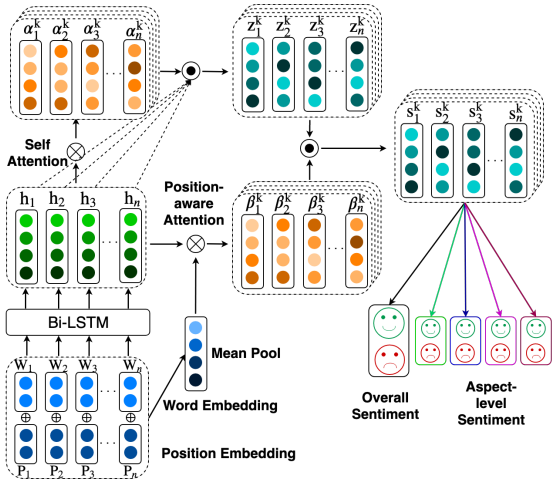
\includegraphics[keepaspectratio, width=0.5\textwidth]{pics/3.png}}
\caption{A representation of the model used by Y. Qiang et al.}
\label{fig}
\end{figure}

The authors provide 2 datasets, one for hotel ratings and the other for restaurant ratings, which they have produced by scraping reviews from TripAdvisor. As shown in Figure 3, the MAN model consists of a number of modules. In the model, the sentences are embedded into word vectors those vectors are combined with their positional information. The input is then parsed into a Bi-LSTM to produce hidden states for each word. Self-attention is then performed to produce alignment vectors for each word for each aspect which are combined with the original hidden states to produce the context vectors for each word.

Position-aware self attention is also performed as words which are closer to an aspect will have more relevance to it usually. These arrays of vectors are also produced for each aspect. Thus we get another set of position-aware alignment vectors. These are combined with the context vectors to give the final representations of the aspects which can then be classified. The classification is performed overall as well as on each aspect on a positive or negative class bases.

Several standard pre-processing techniques, such as lemmatization, stemming, stop word removal and tokenization are used so as to reduce the number of words and to make the process more efficient. Also, the attention scores are used to derive the more important aspects from a text, which is then used to give more weight to it when calculating the overall polarity.

\begin{table}[htbp]
\caption{Results of the model produced by Y. Qiang et al.}
\begin{center}
\begin{tabular}{|c|c|c|c|}
\hline
\multicolumn{2}{|c|}{\textbf{Restaurant}} & \multicolumn{2}{|c|}{\textbf{Hotel}} \\
\hline
\textbf{ACC} & \textbf{Macro-F1} & \textbf{ACC} & \textbf{Macro-F1} \\
\hline
89.64±0.18 & 77.60±0.26 & 83.06±0.14 & 79.81±0.22 \\
\hline
\end{tabular}
\end{center}
\end{table}

From the results above we can see that the model produced sufficiently high accuracy given the fact that the input data was unstructured and scraped off from a review website. And this paper has been successful in addressing the cold-start problem which it aimed to solve. Furthermore, it has introduced a method to build end-to-end ABSA solutions for unstructured data, which without doubt will be expanded upon in the future.\\

\textit{\textbf{Aspect-based Sentiment Analysis with
Type-aware Graph Convolutional Networks and Layer Ensemble, Y. Tian et al., 2021.}}

This paper talks about a better way of using dependency parsing in ABSA. Previous implementations have used dependency graphs for text to assist in performing ABSA for that text, but only the dependencies have been paid attention to, not the exact type of dependency among the words. Clearly some dependencies such as the one between a noun and a verb in a simple sentence are more important in ascertaining the polarity of an aspect within a text as compared with other dependencies that exist within that sentence. If all dependencies are treated equally, this will clearly be a disadvantageous for the model in performing ABSA.

Additionally, this paper claims that although previous Graph Convolutional Networks (GCNs) have learned relations using multiple layers, they only use the result from the most recent layer for ABSA which leads to some being lost because different contextual information is present in different layers in an ensemble.

This paper investigates a Type-Aware Graph Convolutional Network (T-GCN) with multiple layers incorporating both word relational information and dependency type information so as to improve on the current approaches for ABSA. The overall architecture for their approach is given by Figure 4.

\begin{figure}[htbp]
\centerline{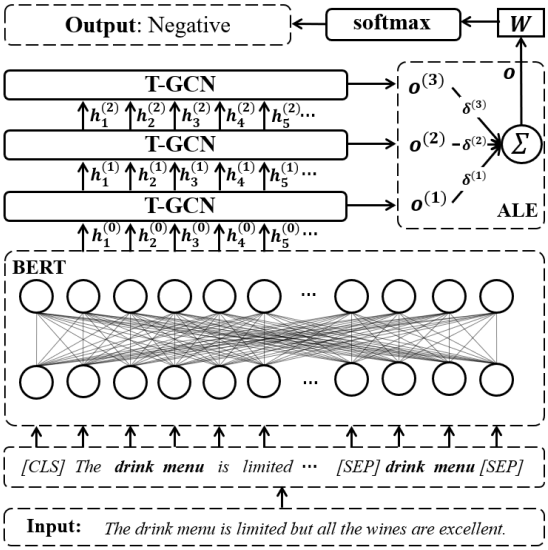
\includegraphics[keepaspectratio, width=0.5\textwidth]{pics/4.png}}
\caption{The overall representation of the model used by Y. Tian et al.}
\label{fig}
\end{figure}

First, given an input sentence, off-the-shelf toolkits are used to get the dependency information. From this information an adjacency matrix is made to show the relation information of the dependency graph, and relation matrix is made to show the type information, as shown in Figure 5. The sentence along with the provided aspect information is tokenized and then the resultant words are vectorized and put through a BERT to get the relevant attention information.

\begin{figure}[htbp]
\centerline{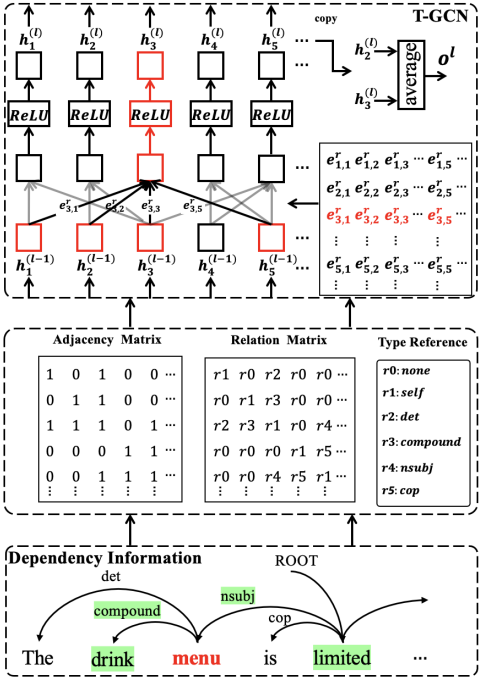
\includegraphics[keepaspectratio, width=0.5\textwidth]{pics/5.png}}
\caption{An illustration of how the type-aware graph is built and how each layer in the T-GCN processes the hidden states.}
\label{fig}
\end{figure}

The graph and the hidden states are then input to the T-GCN where a transition matrix is used to map the relations to their embeddings. For each edge, each layer in the T-GCN first combines the hidden vector with its relational embedding, then the results for the two words connected by the edge are combined and the weight of this edge is calculated. The trainable weight matrix for that layer is then used to produce the intermediate hidden state. Finally, the weight of the edge is applied to the hidden state, and a ReLU activation is performed to produce the hidden state output. This output is then the input for the next layer.

For each word, every layer incorporates information from its connected words into it, this means that multiple layers could learn longer and complex relations. This paper proposes to thus study this contextual information from all the layers using an Attentive Layer Ensemble (ALE). The hidden vectors from each layer are summed and averaged with respect to the number of aspect terms that were initially provided to provide an output from each layer. A weighted average of these output vectors is then taken which is the final output vector for ABSA.

A fully connected layer is then used to map this output vector to the number of classes and then softmax activation is applied to predict the output sentiment for the aspect.

The model showed better accuracy as compared to other famous studies operating on the same datasets. The authors also portrayed which exact studies were utilizing dependency information in their comparison. It is interesting to note that most of the studies with higher performance were using dependency information in some form. This points to the reasoning that exploring the direction of incorporating dependency type information to improve ABSA models might be the direction to go in in the future. The authors have also provided evidence that using T-GCN and ALE both have lead to some improvements in the accuracy of the models.\\

\subsection{2016-2019}

\textit{\textbf{Aspect Level Sentiment Classification with Deep Memory Network, D. Tang et al., 2016.}}

This paper takes inspiration from a question answering using a memory network approach to perform ABSA. The authors have described the problem as searching for a subset of relevant words given an aspect then determining the sentiment of the aspect based on those context words. They claim that their model is better than feature-based Support Vector Machines (SVMs) and attention-based Long Short Term Memory network (LSTM) architectures.

\begin{figure}[htbp]
\centerline{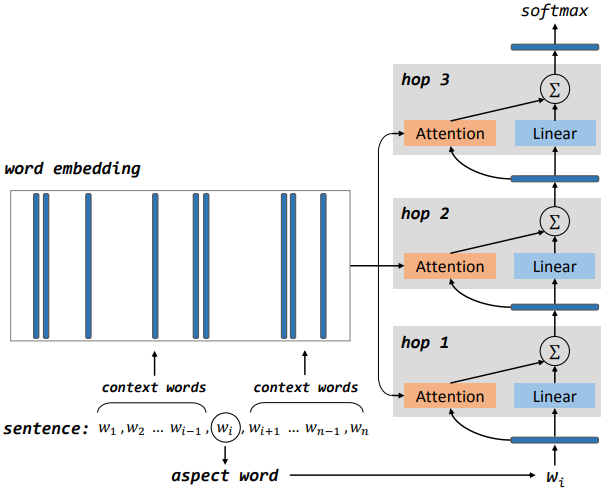
\includegraphics[keepaspectratio, width=0.5\textwidth]{pics/6.png}}
\caption{A representation of the architecture of the model used by D. Tang et al. in their study.}
\label{fig}
\end{figure}

\begin{figure*}
\centerline{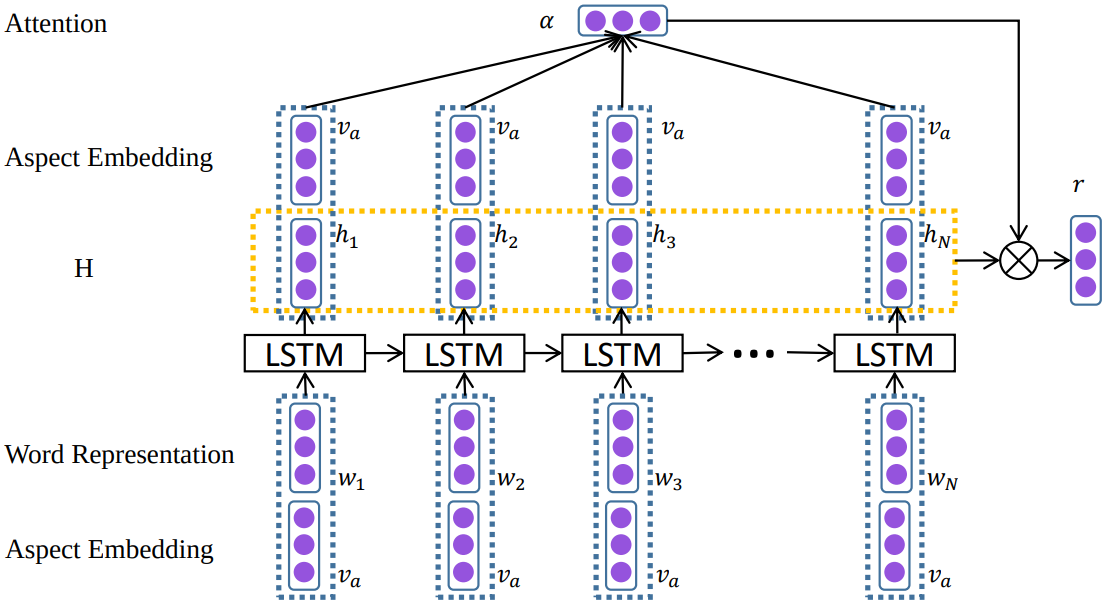
\includegraphics[keepaspectratio, width=\textwidth]{pics/7.png}}
  \caption{A representation of the model used by Y. Wang et al. in their study.}
\end{figure*}

A memory network is a general machine learning framework which comprises of a long-term memory component which can be read and written to and used to help with the task of prediction. A memory network consists of a memory $m$ (which is an array $m$ arrays) and four components $I$, $G$, $O$, and $R$. $I$ converts an input to internal feature representation, $G$ updates the old memory with new input, $O$ generates the output representation given the input and the current memory state, and $R$ converts the output representation to the output.

The model takes in an as input a sentence and an aspect word from that sentence. Each word is then vectorized to produce a word embedding. For the first layer the aspect vector is used as input to select vectors from the memory using attention. The output of the attention and the linearly transformed aspect vector are then combined to produce the input for the next layer. This process is then repeated as shown in Figure 6, until we can then perform a softmax activation on the final output to perform ASC for the input aspect. Like most models, this model uses backpropogation with stochastic gradient descent to train the network weights.

It has become widely accepted that models with multiple layers are able to learn more abstract representations of data. That is the idea behind using multiple "hops" in the model, so that the model can learn more abstract relations between the words and the aspect to get a more accurate measure of the sentiment for an aspect.

\begin{table}[htbp]
\caption{Runtime (seconds) of each training epoch on the Sem Eval 2014 restaurant dataset. The number in the bracket is the number of hops.}
\begin{center}
\begin{tabular}{|c|c|}
\hline
\textbf{Model} & \textbf{Runtime} \\
\hline
LSTM & 417 \\
TDLSTM & 490 \\
TDLSTM + ATT & 520 \\
\hline
MemNet (3) & 9 \\
MemNet (6) & 24 \\
MemNet (9) & 29 \\
\hline
\end{tabular}
\end{center}
\end{table}

Though the accuracy improvement of this work is not very substantial over the best models of this time which were attention-based LSTMs and feature-based SVMs, there was still a slight improvement in accuracy. The more important achievement of this paper is in fact the performance improvement where it takes the model mentioned above substantially less time to train each epoch as compared to the above mentioned models. This comparison is shown in Table 3. It is noticeable how this paper in 2016 was closing in to the self-attention models that were used later on in transformer based architectures.\\

\textit{\textbf{Attention-based LSTM for Aspect-level Sentiment Classification, Y. Wang et al., 2016.}}

This paper takes inspiration from the attention mechanism being introduced to the many domains of NLP, for example Bahdanau et al. in 2014 when they introduced it to the task of Machine Translation. This paper sought to apply those learnings to the domain of ABSA.

In this paper, the authors propose an Attention-based LSTM with Aspect embeddings for the ASC task. Thus, they are proposing to add 2 new features to the traditional LSTM to improve it for the ASC task. The first is to produce a vectorized embedding for the aspect and join it to the word embeddings for each word when they are input into the LSTM. The second feature which the authors propose is an attention mechanism where the attention for all the produced hidden states is calculated with respect to the aspect that was input along with them. This process is summarized by Figure 7.

The paper wanted the aspect embedding to play a role in computing the attention weights thus the aspect vector was appended to the word vectors so the hidden states have the information of the aspects as well. It was then that the attention for each hidden state was computed with the original aspect vectors. The hidden vectors are then multiplied with the corresponding softmax activated attention scores to produce a weighted hidden representation $r$. $r$ is then used to classify the sentiment of the sentence for the initial given aspect. The loss function used in this model is cross-entropy loss.

This model reported better accuracy results than the other models and approaches that it was being compared with. It was tested on 2 tasks, the first where each sentence was accompanied with a set of specific aspects, and the second where there was a set of general aspects which all the sentences were run on. The model reported slightly better results than the model it was being compared against but it should be noted that it did not offer very significant improvements in either task.

It should still be pointed out that this paper introduced the concept of Attention to the problem of ABSC, which then led to further improvements in the coming years.\\

\textit{\textbf{An Unsupervised Neural Attention Model for Aspect Extraction, R. He et al., 2017.}}

This paper identifies 2 main subtasks for AE: (1) extracting the aspect terms from a corpus (such as 'beef', 'rice', 'decor'), and (2) clustering aspect terms into categories (such as 'food', 'service', 'price'). This paper further categorizes the approaches for AE into 3 categories: rule-based, supervised, and unsupervised. Rule-based methods do not usually group aspect terms into categories. Supervised learning methods require data annotation and suffer from domain adaptation problems (cold-start problem as defined above). Unsupervised methods do not need annotation and can derive the aspects from the text directly.

The popular approaches for AE at the time of this paper relied on Latent Dirichlet Allocation (LDA). LDA-based models had the limitation that the individual aspects inferred are often of poor quality. This work attempts to overcome the weaknesses of LDA-based methods by starting with neural word embeddings that map co-occurring words within the same context to nearby points in the embedding space. Then the word embeddings are filtered using an attention mechanism which is then used to derive the aspect embeddings. The authors refer to their approach as Attention-Based Aspect Extraction (ABAE).

\begin{figure}[htbp]
\centerline{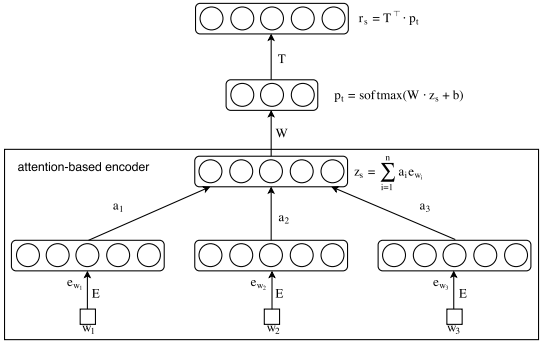
\includegraphics[keepaspectratio, width=0.5\textwidth]{pics/8.png}}
\caption{A representation of the architecture of the model used by R. He et al. in their study.}
\label{fig}
\end{figure}

The approach of this paper is as shown in Figure 8. First the words are transformed into word embeddings, this is beneficial as words that are related are transformed into embeddings that are closer together in the embedding space. Then we use an attention model to calculate the attention of each word. Then we sum up all the word embeddings after multiplying them with their weights to produce the sentence embedding. Once we have the sentence embedding, we reduce that vector by using dimensionality reduction to the number of aspect embeddings. Then the model uses the aspect embeddings to compute the reconstruction of the sentence embedding from the aspect embeddings. The reconstruction describes the aspect as a sum of its aspects. Thus, we first construct an attention-based sentence embedding from the word embeddings, then we extract from it the aspect embeddings so that we can reconstruct the sentence embedding from the aspect embeddings.

The paper correctly concluded a better performance than LDA-based models. However, there was not substantial improvement over the other mainstream models being used such as the $k$-means and the biterm topic model (BTM).\\

\subsection{2012-2015}

\textit{\textbf{Genre Specific Aspect Based Sentiment Analysis of Movie Reviews, V. Parkhe et al., 2015.}}

The aim of this study is to develop a Genre-specific model to perform ABSA on movie reviews. The authors wish to produce an unsupervised aspect based model to analyze the reviews by using a context, that is genre specific lexicons. Thus, they have used separate lexicons for each genre to better predict the sentiments being expressed in the reviews.

\begin{figure}[htbp]
\centerline{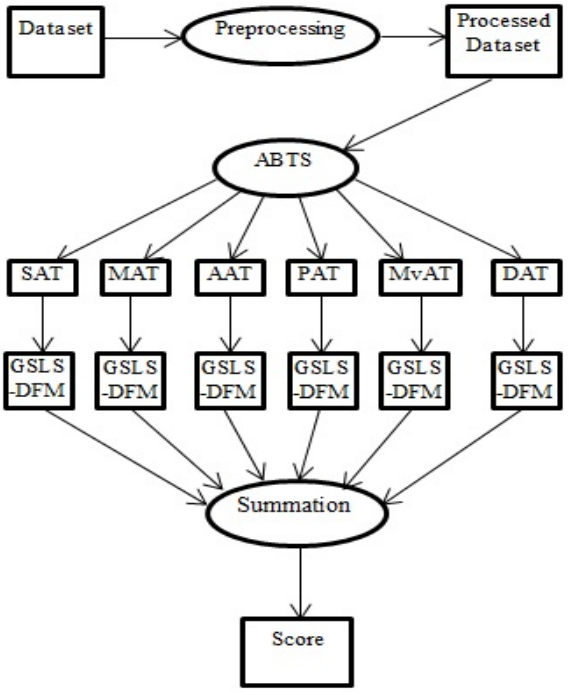
\includegraphics[keepaspectratio, width=0.5\textwidth]{pics/9.png}}
\caption{A representation of the model made by V. Parkhe et al. in their study. ABTS = aspect based text separator, SAT = screenplay aspect text, MAT = music aspect text, AAT = acting aspect text, PAT = plot aspect text, MvAT = movie aspect text, DAT = direction aspect text, GSLS-DFM = genre specific lexicon based scoring and driving factor multiplication.}
\label{fig}
\end{figure}

The architecture of their approach is described by Figure 9. There were a few issues with the dataset that was used in this study due to which a preprocessing step was required. The authors even had to rely on a separate dataset to for the movie ratings to measure their predictions against as the dataset which they were using only had the text review and no numeric rating or score.

The review text is segmented to produce the different texts as described in Figure 9. ABTS not only takes care of the text separation, but also considers the problem of ambiguity in deciding the class a text segment should belong to. To score all of these separated out texts, the authors showed the realization that the same word can describe a different connotation if used to describe movies of different genres. A list of 500 such common words was made and an orientation score was assigned to each of them for each genre using a method called semantic orientation.

Semantic orientation for a given word, is calculated by finding out the difference between the joint information of the word and some positive oriented words, and the joint information of the word and some negative oriented words. Thus the semantic orientation of a word shows its sentiment. In a given text, this is calculated for each word to produce the genre specific score for each category of text. These are then combined to produce an overall score for the review of a movie.

There was variation in the performance of this model over the categories. For example the model performed much better for the `Drama' genre as compared to the `Horror' genre. Furthermore, though this approach is claimed to be unsupervised, any attempt of adapting this same approach would require too much added effort to be a very feasible solution. But, given that this model is a statistical model and not a neural one, the performance is still reasonable.\\

\textit{\textbf{Aspect Based Sentiment Analysis using Support Vector Machine Classifier, R. Varghese et al., 2013.}}

This paper combines the use of dependency parsing, co-reference resolution, SentiWordNet, and an SVM to achieve its goal of aspect-based sentiment analysis. Figure 10 summarizes the sentiment analysis model presented in this paper. The study is conducted on reviews about selected digital cameras from popular websites such as Amazon.in and ebay.in.

\begin{figure}[htbp]
\centerline{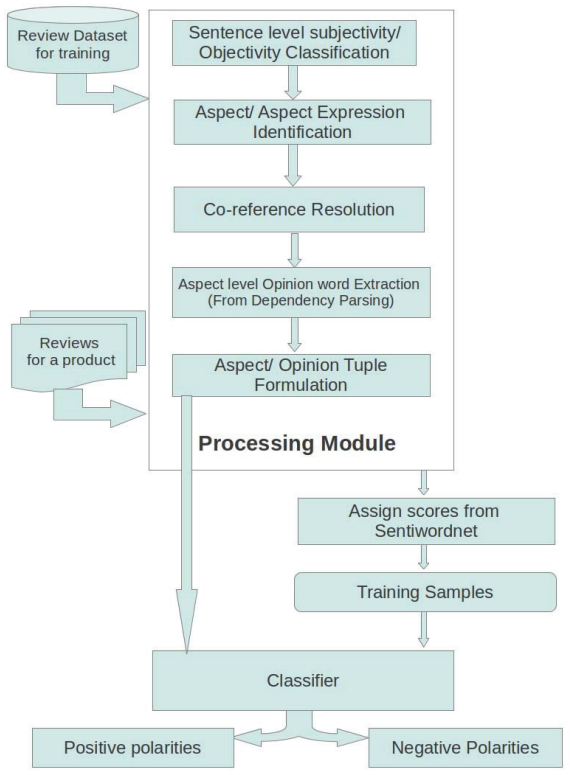
\includegraphics[keepaspectratio, width=0.5\textwidth]{pics/10.png}}
\caption{The sentiment analysis model presented by R. Varghese et al. in their study.}
\label{fig}
\end{figure}

This study presents the idea that a review can sometimes contain sentences which do not present relevant information and should be filtered out so as to reduce the processing overhead. SentiWordNet, which is lexicon library is used for this purpose. The authors have used part-of-speech (POS) tagging to discover the relevant aspects from the text. The training process is used to refine selecting features from the text and discard the non-aspect nouns and features.

This paper proposes the use of co-reference resolution to replace words that are talking about an aspect word with that aspect word itself to help with the classification. This will obviously lead to better classification results for each aspect. They use the Stanford Dependency Parser to extract opinion words and find out which aspect they are related to. Thus the dependency information is used in conjunction with the aspect information to produce the classification. SentiWordNet also helps with assigning opinion or score weights to the extracted opinion to help with the final scoring process.

Finally a SVM is used to classify the sentiment for each aspect. The approach generated reasonably high accuracies given the fact that it was using a just an SVM for the classification. This is due to the fact that the preprocessing steps have been effective in drawing out better relations to make it easier for the classifier to perform its job.\\

\textit{\textbf{Weakly Supervised Joint Sentiment-Topic Detection from Text, C. Lin et al., 2012.}}

The most common approach for SA and ABSA at the time of this paper was LDA as mentioned in the previous review. This paper proposes to extend the LDA approach by adding an additional sentiment layer. The new model is referred to as the weakly supervised joint sentiment-topic (JST) model.

JST was distinguished from the other ABSA models at the time in that it is weakly supervised, so the only supervision comes from a domain independent sentiment lexicon, and that it can detect aspects and sentiments simultaneously. The authors believed that it's weakly supervised nature would make it portable to other domains of SA. The idea behind JST was that aspects are generated based on the sentiment distributions and the words are generated based on the sentiment-aspect pairs.

The existing LDA model is based on the assumption that a document is a mixture of aspects and each aspect is a probability distribution over words. The LDA model goes through the document and calculates the probability for each word to belong to a certain topic given the document (from a predetermined list of topics). Figure 11 gives a graphical representation of the JST model.

\begin{figure}[htbp]
\centerline{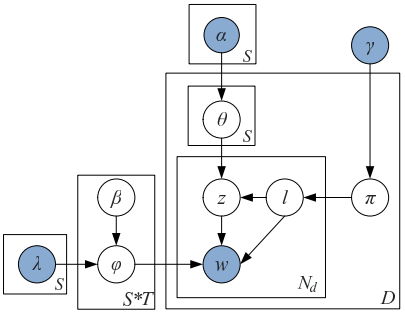
\includegraphics[keepaspectratio, width=0.5\textwidth]{pics/11.png}}
\caption{A graphical representation of the JST model made by C. Lin et al. in their study.}
\label{fig}
\end{figure}

It starts with $S$, the distinct sentiment labels, $T$, the topics, and $D$, a collection of documents. Each document is a list of words from a vocabulary $V$. First, we make a distribution of words for each sentiment-topic pair using the vocabulary. For each document we select a distribution of sentiment labels, then for each label under that document we select a distribution sentiment-topic pairs. Then for each word we select a sentiment label, then a topic, then finally a word from a distribution of words that are related to that topic and sentiment label. Thus, for a given document, its contained topics (aspects) and their sentiments are derived.

This model is an extension and improvement over the baseline LDA model. And as per the results quoted, it does show a significant improvement over the baseline LDA model on the same datasets. The authors also experimented with a reverse-JST model which selected a topic and then a sentiment instead of the other way around. reverse-JST showcased similar results to the JST model.\\

\subsection{2011 and Before}

\textit{\textbf{Multi-aspect Sentiment Analysis with Topic Models, B. Lu et al., 2011.}}

This paper first describes 2 tasks related to ABSA to investigate. The first is multi-aspect sentence labeling where each sentence in a document is labeled according to the aspects it contains. This can be thought of being a sentence level aspect extraction of sorts. They have proposed a weakly supervised topic modeling approach for this. The second task is multi-aspect rating prediction where the aspect ratings for each review are predicted. A supervised approach using the labeled values and an unsupervised approach using the first task are both experimented on.

4 types of topic models are used to experiment on these approaches. These are: LDA, Local LDA (L-LDA), Multi-grain LDA (MG-LDA), and Segmented Topic Model (STM). The last of these was a relatively new approach which had not been used on sentiment analysis tasks.

\begin{figure}[htbp]
\centerline{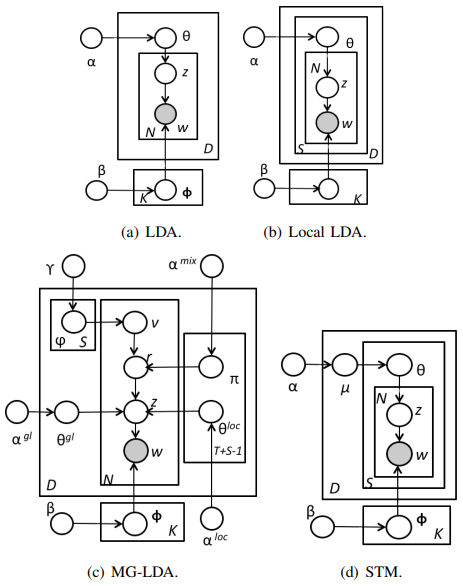
\includegraphics[keepaspectratio, width=0.5\textwidth]{pics/12.png}}
\caption{A overview of the architecture of the topic models being used}
\label{fig}
\end{figure}

Simply put, topic models want to capture word co-occurrence information to understand hidden topics within a model. LDA and L-LDA are based on a probabilistic generative model which assumes that documents are mixtures over topics. Formally they assume the corpus is generated according to the following:
\begin{itemize}
\item For each topic $k$:
  \begin{itemize}
  \item Choose word-topic mixture $\phi_k \sim Dir(\beta)$
  \end{itemize}

\item For each document $d$:
  \begin{itemize}
  \item Choose document topic proportions $\theta_d \sim Dir(\alpha)$
  
  \item For each word $w$ in document $d$:
    \begin{itemize}
    \item Choose topic $z_{d,w} \sim \theta_d$
    \item Choose word $w \sim \phi_{z_{d,w}}$
    \end{itemize}
  \end{itemize}
\end{itemize}
L-LDA are only different from LDA by them modeling the sentences as documents.

In response to the limitations of the above, MG-LDA models were made which aim to model global topics to correspond to local topics. This can be thought of as the global topics being broad categories and the local topics being items corresponding to those categories. Finally, STM aims to jointly model document and sentence-level topic proportions by using a Poisson Dirichlet Process (PDP). This works as follows:
\begin{itemize}
\item Choose document topic proportions $\theta_d \sim Dir(\alpha)$

\item For each sentence $s$:
  \begin{itemize}
  \item Choose topic proportions $\theta_s \sim PDP(\theta_d, a, b)$
  \end{itemize}

\item For each word $w$ in sentence $s$:
  \begin{itemize}
    \item Choose topic $z_{d,w} \sim \theta_s$
    \item Choose word $w \sim \phi_{z_{d,w}}$
  \end{itemize}
\end{itemize}
It can be clearly seen that STM is just an extension of L-LDA that takes into account document level topic distributions instead of just sentence level ones.

For the labeling task, L-LDA was the best performing model out of the 4 compared, but it should be noted that even that did not perform as well as an SVM based model. For the rating prediction task, LDA and L-LDA were the best performing models. They noted that though these models can help some weaker machine learning models in prediction, the performance improvement is negligible for stronger machine learning models.\\

\textit{\textbf{Aspect-Based Opinion Polling
from Customer Reviews, J. Zhu et al., 2011.}}

This paper explores the task of performing ABSA on free-form text reviews by dividing it into 3 parts: (1) using a Multi-aspect bootstrapping method to learn aspect-related terms from unlabeled data for each given aspect, (2) using an aspect-based sentence segmentation model to divide the sentence into multiple single aspect parts, and (3) passing these segments into an opinion polling algorithm to produce a sentiment for each segment.

This paper talks about a statistical approach to the ABSA problem rather than the many neural or machine learning approaches of today (reasonably so as this was published in 2011). So given a finite set of aspects $A$, a finite set of polarities $P$, a set of $n$ customer reviews $X$, and a score function $\phi$ giving a voting score for each pair $(a,p) \in A \times P$; the goal is to calculate:
\begin{equation*}
  \phi (a,p|X) = \frac{\sum_{1 \leq i \leq n} \phi (a,p|x_i)}{n}
\end{equation*}
which is the score for every pair of aspect and polarity for each sentence in the corpus.

As the goal of this study is to perform ABSA on unlabeled data without using a machine learning model, they are using a dictionary of keywords to learn the aspect-related terms for each aspect. This is then used to later learn the aspect terms from each sentence. The way this is performed is first some specified aspect-related seed terms are selected based on relevance to the dataset. Then the best terms related to those seed words are selected to form a candidate set. Then using a separate scoring function the best terms from the candidate list are added to the initial seed set to give us our list of words for a particular aspect $a$. The algorithm repeats this process for all the aspects. A score vector is produced for each aspect term corresponding to the set of aspect related terms.

Then the model identifies the aspects in each segments. Given a sentence, an ambiguity score for each aspect term from each aspect with respect to the sentence is calculated. Using this the most probable aspects for a sentence can be identified. As a sentence can contain more than one aspects, a segmentation of a sentence over the most likely aspects is calculated, and then the sentence is segmented accordingly. Then we just use the segments and its identified aspect to produce a sentiment for each segment given its aspect.

The results of this model are not very impressive as compared to the neural models that we have seen so far, but that does not discredit the statistical and algorithmic approach that has been described in this model. For example it might be invaluable for some applications to think of the sentence in term of it's constituent segments and perform a simpler sentiment analysis on them than to think of it in a more complicated way. Furthermore, this paper does successfully describe a semi-supervised approach to the ABSA problem using a relatively simple methodology which is a challenge which ABSA still faces today.\\

\textit{\textbf{Sentiment Analyzer: Extracting Sentiments about a Given Topic using Natural Language Processing Techniques, J. Yi et al., 2003.}}

This paper introduces a very early approach to perform ABSA. It correctly identifies the needs and the motivation to perform ABSA, which with time have only grown. This can be seen by the fact that in the 20 years after the publication of this paper, the statements regarding the need for ABSA have only become truer.

This paper introduces a statistical model that takes in a document and extracts from the document topic-specific features. It then extracts all the opinion bearing phrases from the document and deduces their sentiment. Finally it makes the (topic$\mid$feature, sentiment) relations. For example, for the domain of digital camera, a feature is a part of the camera such as the lenses, a feature of the camera such as the price, or a feature of a part of the camera such as the battery life.

The paper identifies that the feature terms are usually nouns and then focuses on these for the feature term extraction algorithm. They tested 3 heuristics for candidate term selection: Base Noun Phrases (BNP),  Definite Base Noun Phrases (dBNP), and Beginning Definite Base Noun Phrases (bBNP). The paper develops 2 algorithms to perform feature extraction, one based on a mixture language model and the other based on likelihood ratio.

In the first algorithm, the authors note that a document can be considered to be generated by a linear combination of the general web language model $\theta_W$ (similar to the corpus language model), and the  topic-specific language model $\theta_T$ (similar to the query model):
\begin{equation*}
  \theta = \alpha \theta_W + \beta \theta_T
\end{equation*}
where $\theta$, $\theta_W$, and $\theta_T$ are multidimensional distributions over the number of words in the corpus. The idea is to calculate the $\theta_{T_i}$ score for each term in a document. Then the feature terms with their score satisfying some confidence level are selected. For the likelihood test algorithm, we compute the likelihood score for each candidate feature term, and then select the terms which satisfy some confidence level.

\begin{figure}[htbp]
\centerline{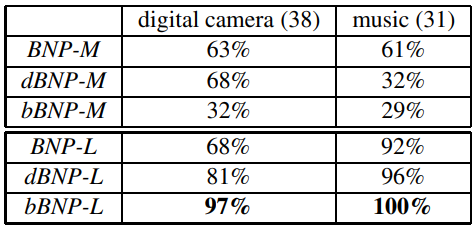
\includegraphics[keepaspectratio, width=0.5\textwidth]{pics/13.png}}
\caption{A comparison of the precision of the different feature term extraction algorithms over the digital camera and the music corpora.}
\label{fig}
\end{figure}

As can be seen from Figure 13, the bBNP heuristic with the likelihood score algorithm yielded the best accuracy for feature term extraction.

The actual sentiment analysis part of the feature terms is done by using a sentiment pattern database which matches patterns in the text to defined sentiment patterns and assigns the matches sentiments accordingly. It is easy to see that this statistical approach is a rather primitive compared to the powerful neural models of today and that it will suffer from very high domain adaptability issues and that it might suffer from input such as customer reviews which use informal expression and language which will will make it difficult to capture all sentiment patterns that can occur.

That being said it still performs relatively well on general web documents and news articles as indicated by the results obtained. This points to the ingenuity of this idea of performing ABSA with very limited resources for the time using a statistical model.

\section{Conclusion}

Therefore we have seen in this survey not only the practices being used for ABSA today, but also older statistics and probability based approaches that were used before neural networks were introduced to the task. We have also explored some methods that have been used to help with the classification steps such as using word relation information, and processing the input to make it easier to extract the aspects. From this we can now appreciate the efforts that have been made in this field.

\begin{thebibliography}{00}
\bibitem{b1} A. Karimi, L. Rossi and A. Prati, "Adversarial Training for Aspect-Based Sentiment Analysis with BERT," 2020 25th International Conference on Pattern Recognition (ICPR), Milan, Italy, 2021, pp. 8797-8803, doi: 10.1109/ICPR48806.2021.9412167.
\bibitem{b2} Y. Qiang, X. Li and D. Zhu, "Toward Tag-free Aspect Based Sentiment Analysis: A Multiple Attention Network Approach," 2020 International Joint Conference on Neural Networks (IJCNN), Glasgow, UK, 2020, pp. 1-8, doi: 10.1109/IJCNN48605.2020.9207426.
\bibitem{b3} Yuanhe Tian, Guimin Chen, and Yan Song. 2021. Aspect-based Sentiment Analysis with Type-aware Graph Convolutional Networks and Layer Ensemble. In Proceedings of the 2021 Conference of the North American Chapter of the Association for Computational Linguistics: Human Language Technologies, pages 2910–2922, Online. Association for Computational Linguistics.
\bibitem{b4} Duyu Tang, Bing Qin, and Ting Liu. 2016. Aspect Level Sentiment Classification with Deep Memory Network. In Proceedings of the 2016 Conference on Empirical Methods in Natural Language Processing, pages 214–224, Austin, Texas. Association for Computational Linguistics.
\bibitem{b5} Yequan Wang, Minlie Huang, Xiaoyan Zhu, and Li Zhao. 2016. Attention-based LSTM for Aspect-level Sentiment Classification. In Proceedings of the 2016 Conference on Empirical Methods in Natural Language Processing, pages 606–615, Austin, Texas. Association for Computational Linguistics.
\bibitem{b6} Ruidan He, Wee Sun Lee, Hwee Tou Ng, and Daniel Dahlmeier. 2017. An Unsupervised Neural Attention Model for Aspect Extraction. In Proceedings of the 55th Annual Meeting of the Association for Computational Linguistics (Volume 1: Long Papers), pages 388–397, Vancouver, Canada. Association for Computational Linguistics.
\bibitem{b7} C. Lin, Y. He, R. Everson and S. Ruger, "Weakly Supervised Joint Sentiment-Topic Detection from Text," in IEEE Transactions on Knowledge and Data Engineering, vol. 24, no. 6, pp. 1134-1145, June 2012, doi: 10.1109/TKDE.2011.48.
\bibitem{b8} V. Parkhe and B. Biswas, "Genre Specific Aspect Based Sentiment Analysis of Movie Reviews," 2015 International Conference on Advances in Computing, Communications and Informatics (ICACCI), Kochi, India, 2015, pp. 2418-2422, doi: 10.1109/ICACCI.2015.7275981.
\bibitem{b9} R. Varghese and M. Jayasree, "Aspect based Sentiment Analysis using support vector machine classifier," 2013 International Conference on Advances in Computing, Communications and Informatics (ICACCI), Mysore, India, 2013, pp. 1581-1586, doi: 10.1109/ICACCI.2013.6637416.
\bibitem{b10} B. Lu, M. Ott, C. Cardie and B. K. Tsou, "Multi-aspect Sentiment Analysis with Topic Models," 2011 IEEE 11th International Conference on Data Mining Workshops, Vancouver, BC, Canada, 2011, pp. 81-88, doi: 10.1109/ICDMW.2011.125.
\bibitem{b11} B. Lu, M. Ott, C. Cardie and B. K. Tsou, "Multi-aspect Sentiment Analysis with Topic Models," 2011 IEEE 11th International Conference on Data Mining Workshops, Vancouver, BC, Canada, 2011, pp. 81-88, doi: 10.1109/ICDMW.2011.125.
\bibitem{b12} J. Yi, T. Nasukawa, R. Bunescu and W. Niblack, "Sentiment analyzer: extracting sentiments about a given topic using natural language processing techniques," Third IEEE International Conference on Data Mining, Melbourne, FL, USA, 2003, pp. 427-434, doi: 10.1109/ICDM.2003.1250949.
\end{thebibliography}
\end{document}